\documentclass[journal]{vgtc}                % final (journal style)

\usepackage{indentfirst} %MCW added

%% These few lines make a distinction between latex and pdflatex calls and they
%% bring in essential packages for graphics and font handling.
%% Note that due to the \DeclareGraphicsExtensions{} call it is no longer necessary
%% to provide the the path and extension of a graphics file:
%% \includegraphics{diamondrule} is completely sufficient.
%%
\ifpdf%                                % if we use pdflatex
  \pdfoutput=1\relax                   % create PDFs from pdfLaTeX
  \pdfcompresslevel=9                  % PDF Compression
  \pdfoptionpdfminorversion=7          % create PDF 1.7
  \ExecuteOptions{pdftex}
  \usepackage{graphicx}                % allow us to embed graphics files
  \DeclareGraphicsExtensions{.pdf,.png,.jpg,.jpeg} % for pdflatex we expect .pdf, .png, or .jpg files
\else%                                 % else we use pure latex
  \ExecuteOptions{dvips}
  \usepackage{graphicx}                % allow us to embed graphics files
  \DeclareGraphicsExtensions{.eps}     % for pure latex we expect eps files
\fi%

\usepackage{microtype}                 % use micro-typography (slightly more compact, better to read)
\PassOptionsToPackage{warn}{textcomp}  % to address font issues with \textrightarrow
\usepackage{textcomp}                  % use better special symbols
\usepackage{mathptmx}                  % use matching math font
\usepackage{times}                     % we use Times as the main font
\renewcommand*\ttdefault{txtt}         % a nicer typewriter font
\usepackage{cite}                      % needed to automatically sort the references

%% Paper title.
\title{Investigation Into Cryptocurrency Pricing Patterns With Respect to Financial Instability \\
CS 725/825, Fall 2017}

%% This is how authors are specified in the journal style

%% indicate IEEE Member or Student Member in form indicated below
\author{Jason Orender\\
Department of Computer Science\\
Old Dominion University\\
Norfolk, VA 23529\\
jorender@cs.odu.edu
}
\authorfooter{
}

%other entries to be set up for journal
\shortauthortitle{Jason Orender \MakeLowercase{\textit{et al.}}: Cryptocurrency Pricing Patterns}
%\shortauthortitle{Firstauthor \MakeLowercase{\textit{et al.}}: Paper Title}

%% Abstract section.
\abstract{Pricing patterns with respect to cryptocurrencies and their motivations have been the subject of heated debate among investment professionals and academicians alike\cite{ftepper-1,rviglione-1}.  The purpose of this visualization is to provide a focused presentation of the world events conincident with spikes in peer-to-peer cryptocurrency transactions together with a continuous evolutionary timeline to provide perspective regarding the state of development and usage at a national, regional and worldwide level.  As a matter of practical concern, Bitcoin was the sole cryptocurrency used in this analysis due to the large amount of country specific peer-to-peer data available, as well as the relatively simple purpose for which it is intended - namely, the transfer of monetary value from one individual to another.   %
} % end of abstract

%% Uncomment below to include a teaser figure.
\teaser{
	\centering
	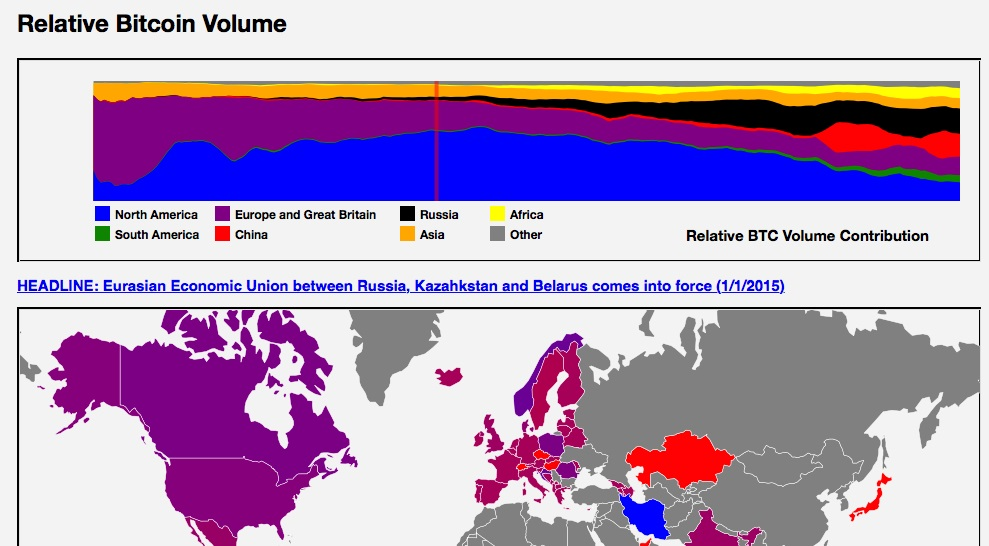
\includegraphics[width=0.7\linewidth]{teaser_1}
	\caption{Bitcoin adoption as a function of time shows an increasingly global shift.  What was once the province of western nations almost exclusively, has now become a worldwide phenomenon. This visualization is intended to give some insight concerning why. }
	\label{fig:teaser}
}

%% Uncomment below to disable the manuscript note
\renewcommand{\manuscriptnotetxt}{}

%% Copyright space is enabled by default as required by guidelines.
%% It is disabled by the 'review' option or via the following command:
 \nocopyrightspace

\vgtcinsertpkg

%%%%%%%%%%%%%%%%%%%%%%%%%%%%%%%%%%%%%%%%%%%%%%%%%%%%%%%%%%%%%%%%
%%%%%%%%%%%%%%%%%%%%%% START OF THE PAPER %%%%%%%%%%%%%%%%%%%%%%
%%%%%%%%%%%%%%%%%%%%%%%%%%%%%%%%%%%%%%%%%%%%%%%%%%%%%%%%%%%%%%%%%

\begin{document}

%% The ``\maketitle'' command must be the first command after the
%% ``\begin{document}'' command. It prepares and prints the title block.

%% the only exception to this rule is the \firstsection command
\firstsection{Introduction}

\maketitle

The reasons for the rise and fall of the exchange rate of cryptocurrencies provoke a wide variety of explanations\cite{ftepper-1,rviglione-1}, and with as many as 1,110 currencies in circulation\cite{ditkis-1} a coherent explanation can be hard to find.  The motivation for pricing CannabisCoin\cite{alex-1}, for instance, is far different from the pricing mechanism for Bitcoin.  For that reason, I made the choice to focus on Bitcoin purely as a means for storing and transferring value from one individual to another.  To this end, I downloaded the Bitcoin and local Fiat Currency exchange volumes from the LocalBitcoins data set for all 46 countries represented on the Coin.Dance website\cite{coind-1}.  This data was normalized and coordinated with data from contemporary news headlines harvested via Google search.  

The time range of interest starts in August of 2013 and continues through November of 2017. The widest possible aperture was desired, but the level of adoption simply was not robust enough to provide consistent data prior to August 2013.

Answering the fundamental question of what, if any, effects on global or local Bitcoin pricing are due to newsworthy events is the primary goal of this visualization.  Identifying the effects of local instability on exchange volume as well as whether periods of relative calm coincide with negative price correlation are secondary but integrated goals.

The abstract tasks for this visualization branch from the 
\begin{equation}\label{key}
Analyze \rightarrow Consume \rightarrow Present 
\end{equation}
framework.  Specifically, I used:

\begin{equation}\label{key}
Search \rightarrow  Locate \rightarrow Query \rightarrow Identify
\end{equation}
by using Bitcoin trading volume to locate areas of interest and then used that location to research headline data and identify possible causes.

And also: 
\begin{equation}\label{key}
Search \rightarrow Explore \rightarrow Query \rightarrow Summarize Cross-Correlations
\end{equation}
by using spikes in trading volume along with comprehensive evolutionary data from both the exchange rate area graph and the relative contribution stacked area graph to draw conclusions about the effect of worldwide and local events on exchange rate.

\section{Related Work}

There is very limited work in this area due to the relatively new nature of cryptocurrencies in general.  Robert Viglione of the University of South Carolina \cite{rviglione-1} has done some work in this area for his PhD dissertation.  He concentrated on the correlations between economic freedom and Bitcoin pricing, though the questions that he posed were somewhat more narrow than the ones posed in this paper. He examined the Bitcoin price premium specifically in countries with known repressive regimes as quantified by the Heritage Foundation Economic Freedom Index \cite{heritage-1}.

\begin{figure}[tb]
 \centering % avoid the use of \begin{center}...\end{center} and use \centering instead (more compact)
 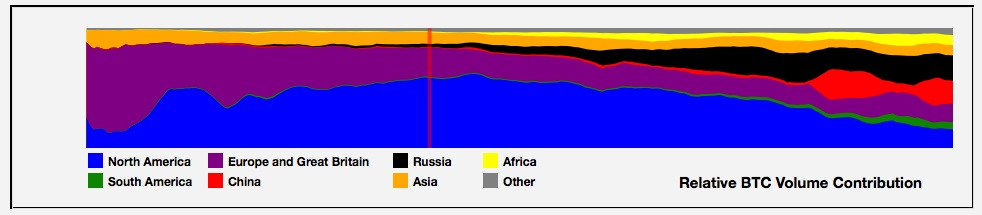
\includegraphics[width=\columnwidth]{stacked_area}
 \caption{The stacked area graph showing the relative contribution of each geographic area over the entirety of the dataset.}
 \label{fig:sample}
\end{figure}

\section {Data}
The data used for this visualization was collected primarily from the Coin.Dance \cite{coind-1} website.  This website harvests data weekly from the LocalBitcoins trading platform and collates it in the form of a variety of charts and graphs.  The site has a download option for a comma-separated-value (csv) file with the data for each of their charts.  This is the function that I used to collect my data from their country specific volume charts. The data for both the Bitcoin volume and the country specific fiat currency volume was collected.  Dividing the Bitcoin volume into the fiat currency volume also provided a de-facto exchange rate. 

\begin{equation}\label{key}
E_{n,i} = \frac{F_{n,i}}{V_{n,i}}
\end{equation}
where:\\
$ E_{n,i} = $ Exchange rate for the currency of country 'i' in week 'n'\\
$ F_{n,i} = $ Fiat currency volume of country 'i' in week 'n'\\
$ V_{n,i} = $ Bitcoin volume of country 'i' in week 'n'\\

 This was extremely useful since many of the countries of interest do not publish a realistic government sponsored exchange rate.  Venezuela, for instance, has a complex system of four exchange rates, the most generous of which was 200 bolivars per dollar as of January, 2016 \cite{edisilvestro-1}.  LocalBitcoins data would suggest that no one in-country would be willing to part with a US Dollar at that time for anything less than 717 bolivars per dollar - a significant discrepancy.  As a point of reference, the latest data via LocalBitcoins at the end of November, 2017 puts the exchange rate at 30,058 bolivars per dollar.  This type of data is unavailable via any official channel.

The LocalBitcoins data was originally viewed as ancillary or supporting data, but as I delved into the problem I realized that it might actually represent a more objective level of data than the others that might be available; this is due to the fact that it simply represents the amount that an individual on the ground in a specific country would be willing to pay for Bitcoin in their local currency.  For that reason, I decided to use it as my primary data set.

Additionally, part of the visualization coordinates headline data with the visual exchange rate and volume data presented on the map and in the charts.  This data was collected via Google search in a systematic manner and is fully linked to each supporting source.  The countries showing the highest volume upticks (marked as red on the map) were searched with the phrase "[COUNTRY] BITCOIN [MONTH] [YEAR]" in order to eliminate any specific Bitcoin related news that might have influenced the price since these events will at the very least muddy the waters enough that a clear conclusion regarding the cause could not be reached.  If there were no significant Bitcoin relevant headlines, the search phrase "[COUNTRY] NEWS [MONTH] [YEAR]" was entered.  If this was not fruitful, a simple query phrase of "[COUNTRY] [MONTH] [YEAR]" was used.  If multiple countries were marked red during the same week, a query phrase of "[COUNTRY-1] [COUNTRY-2] ... [COUNTRY-N] NEWS [MONTH] [YEAR]" was used prior to querying the individual countries.  This occasionally produced interesting news results that affected several countries simultaneously, such as a migrant worker crisis affecting both Sweden and Hungary, for instance.  The relevance of the headlines were subjectively judged by myself, so this will contain a certain amount of bias; however, I attempted to reduce this as much as practical by systematically using the visualization as a guide for which countries to search for relevant news on, and I always prioritized the finds with Bitcoin news first, Finance related news second, and general news third.

The data fields that I ended up with were:
\begin{enumerate}
	\item Bitcoin Exchange Rate (quantitative)
	\item Date (ordinal)
	\item Normalized Fiat Trading Volume (quantitative)
	\item Relative (normalized) Contribution to Bitcoin Volume (quantitative)
	\item Country (categorical)
	\item Headline Data (categorical)
\end{enumerate}

Several of these data fields were derived from the raw data that I harvested from LocalBitcoins:
\begin{enumerate}
	\item Bitcoin Exchange Rate is simply the Bitcoin Volume divided into the Fiat currency volume for a specific country (equation 4). This data was used in the area graph underneath the map.
	\item Normalized Fiat Trading Volume was the Fiat currency trading volume for that week divided by the average of the previous six weeks (exclusive) and then multiplied by 500 and capped at 1,000.  This yielded a number from 0 to 1000, with 500 being average.  This number is used to color the map and is also shown as the light gray line overlaid on the exchange rate area graph (equation 6).
	\item Relative (normalized) contribution to Bitcoin Volume was calculated by adding up all of the Bitcoin volume for that week and dividing it into the Bitcoin volumes for each of the aggregated geographic areas consisting of North America, South America, Europe and Great Britain, China, Russia, Asia, Africa, and all others.  This data is reflected in the stacked area graph shown above the map (equation 5).
\end{enumerate}

\section{Visualization}
This visualization is divided into three parts: a stacked area graph, a choropleth map, and a simple area graph with a superimposed line graph.  All three components are linked and will result in updating the other two when the appropriate area is clicked.  The stacked area graph functions as a comprehensive time line that will also give an indication of where the activity will be concentrated; clicking on a portion of that chart will shift the world map to display a particular week of data.  The world map displays all of the countries of the world color coded to Bitcoin trading activity; clicking on a country will cause the bottom area graph and superimposed line graph to update.  The bottom area graph depicts exchange rate in that country and also has a superimposed line graph that shows relative trading volume; this graph can also act as an interactive timeline and clicking it will update the world map in much the same manner as clicking on the stacked area graph.

As an aside, the linked headline data is nestled between the stacked area graph and the world map.  While not technically part of the visualization, it does provide relevant background on world events during the week in question and is critical to answering the questions posed at the beginning of this paper.

The Map of the world is the centerpiece of the visualization and displays a choropleth map depicting relative levels of trading volume from the local fiat currency to Bitcoin; red is indicative of a high level of activity, blue is indicative of a low level of activity, and purple is average.  There are varying shades in-between these levels reflecting the entire continuum of activity levels.  If any countries either do not have data reflected in the dataset or if the level of activity does not rise to at least 25 percent of the country lifetime average, the country is grayed out.  Preventing countries from displaying until the 25 percent threshold is reached is used to hide the initial wildly varying fluctuations in volume that typically accompany initial adoption of Bitcoin usage in that economy.  This may be of interest to answer other questions, but the primary question that this visualization is trying to answer is whether there is a connection between newsworthy events and Bitcoin exchange pricing; including the initial data would prove distracting and is unlikely to help answer that question.

The stacked area graph positioned over the map of the world provides a comprehensive time line of the entire span of interest and shows relative adoption levels all over the world.  It is notable that this graph shows peer-to-peer transactions, and while this is relevant to answering the particular questions posed in this paper, it excludes official public exchange volume.  In countries where there are large reputable exchanges like the United States (Coinbase), the European Countries (BitStamp), and Japan (BitFlyer) there is less of a need for peer-to-peer transactions.  To illustrate, this phenomenon can be specifically noted in the Chinese area on the graph (red).  Note the rapid expansion over the first half of 2017, the gradual constriction until September and then the rapid expansion again.  The second rapid expansion occurred precisely when the Chinese government took a heavy handed approach and shut down all cryptocurrency exchanges in the country at the beginning of September\cite{cdengpvigna-1}. So, while peer-to-peer volume has indeed continued to climb at a steady rate in the United States, for instance (see the accompanying figure pulled directly from the Coin Dance website), much of the volume that might otherwise be attributed to the United States is not visible in this graph.  In contrast, the graph for China reflects the narrowing shown in the area graph and then rapid expansion again.

\begin{figure}
	\centering
	\includegraphics[width=0.7\linewidth]{USA_coindance}
	\caption{Rising levels of peer-to-peer Bitcoin transactions in the United States\cite{coind-1}}
	\label{fig:usacoindance}
\end{figure}

\begin{figure}
	\centering
	\includegraphics[width=0.7\linewidth]{CHINA_coindance}
	\caption{Relatively small levels of activity, followed by an explosion of growth and then decline as government approved public exchanges rise to prominence.  The second hump occurs simultaneously with the rapid closure of all public exchanges in the country.\cite{coind-1}}
	\label{fig:chinacoindance}
\end{figure}

The area graph underneath the map shows the local exchange rate in the last country selected on the map.  In most cases, the local exchange rate will mirror the shape of the exchange rate in other countries, though the values for the vertical axis will be different, since this is scaled in local currency fiat values.  While the shape is very similar in many countries, the dips and peaks in some countries are exaggerated while the same dips and peaks are muted in others.  The most radical departure from the norm is Venezuela, which shows an unbroken hyperbolic shape from the beginning to the end of the graph.  These departures from the norm are usually reflected in the exchange volume trace, which is overlaid in light gray.  This line depicts a normalized value for exchange volume and can be used to home in on time periods of interest.  When the trace is high, the country should show up as bright red on the map, when the trace is low, the country should show up as a deep blue.

\subsection{Design Decisions}
The domain of interest for this visualization is the effect of notable events on Bitcoin exchange pricing.  Those interested in this domain will likely focus in on one particular geographic area (probably their own), and then branch out to view the effects on other areas of interest.  To that end, I believe that the world map serves as a particularly good starting point and general focus for the visualization.  While presenting a specific set of derived and aggregated data, it is not an exploratory tool, but it gives the illusion of exploration on the part of the user by presenting multiple avenues for navigation through the data.

There are essentially two dimensions being presented with this visualization, time and geographic area.  The entire expanse of time is depicted in the stacked area graph on top of the map, and then also in the area graph and activity trace underneath the graph.  These two presentations provide different features for the user to attend to, but clicking on either one shifts the central map to provide a snapshot of the entire world in that short span of time (a week).

Harkening back to the stated abstract tasks of Analyzing, Consuming and presenting discussed in section 1, it is clear that though the analysis has already been done in the preparation of the visualization, it is needed for the user to be able to look at the visualization and come up with the same conclusions that the visualization was intended to convey.  For this reason, I decided to use the exchange rate versus time in the lower area graph.  Since this is the attribute that has most ignited the public imagination, any visualization that purported to show the evolution of Bitcoin and excluded it would immediately lose user interest.  Since the price appreciation has been widely covered in the media, it is also a good secondary indicator of time.  Later in the time period of interest implies greater exchange rate and thus is the focus of greater interest.  The user can then consume the data presented in the appropriate area of the visualization.

Once the user has analyzed the data presented and searched for the area of interest, they are then able to locate the week of interest.  They will then be able to query that week by clicking on the graph and shifting the map to display data from that week.  They are then able to identify the geographic region of interest after the map shifts and by clicking on that area they can switch the exchange rate graph to this new area of interest.  This is a recursive process that can go on for many iterations as the area and time of interest are refined.

Alternatively, the user can start with the stacked area graph over the map to home in on a time period when the United states dominated the peer-to-peer exchange traffic or when China was a dominant player, for instance.  By providing several different indicators with details about why a particular time period might be of interest, it helps the user to locate the area of interest so that the query can proceed.  What I wanted to avoid was a visualization that presented the user with a variety of disconnected facts and provided no clue regarding the way to proceed.  This was the thought behind the interaction idiom that was ultimately settled on.

The particular visual encoding choices that would be most effective seemed rather straightforward in this case.  Since the stated purpose of the visualization was to draw conclusions regarding the effect of notable events on Bitcoin pricing, it made sense that some of those events might be regional or local in nature and a way to identify the areas of interest was necessary.  Since geography plays such a central role, a choropleth map seemed to be a good choice as a presentation idiom.  Also, since the statistic of interest was Bitcoin value and trading volume as a function of time, either line or area graphs again seemed to be the most comprehensible idiom to convey that information.  An area graph was chosen to represent the exchange rate as opposed to a line simply to make it stand out on the page; a single line is easier to overlook.  In fact this was used to some advantage by including the trace of the trading volume on the same chart as the area graph of the exchange rate.  These are closely related and complimentary statistics, but in order to prevent the chart from looking too busy, the relative volume was added as a light trace.

\begin{figure}
	\centering
	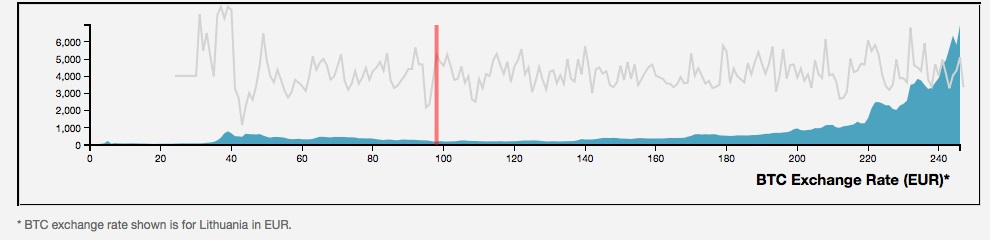
\includegraphics[width=0.9\linewidth]{exchange_rate}
	\caption{The Bitcoin exchange rate chart is shown as a function of time.  The vertical red bar indicates the time period used to populate the choropleth map, the gray line shows relative volume (a high value would be indicated by that country showing up as bright red on the map, while a low value woud be indicated by that country showing up as a deep blue on the map), and the area shows Bitcoin exchange rate in that country. }
	\label{fig:exchangerate}
\end{figure}

\section{Analysis}

This visualization is a relatively simple interaction between three separate idioms: a normalized stacked area chart, a choropleth map, and a simple area chart with a superimposed line chart.  The data is queried by identifying an area or region of interest and then clicking on it to alter the aspect of the data shown in the other charts.\\

\begin{tabular}{|l|l|}
\hline
	What: Data & Table \\ \hline
 	What: Derived & Relative contribution, Exchange Rate, \\&normalized trading volume \\ \hline
 	Why: Tasks & Identify time or location of interest, \\&examine exchange rate response, \\&present relevant news headline \\ \hline
 	How: Encode & Stacked area, area, choropleth map \\ \hline
 	How: Manipulate & Select \\ \hline
 	How: Facet & Coordinated linked response with \\&highlighted time slice.\ \\ \hline
 	Scale & 47 countries over 246 weeks \\ \hline
\end{tabular}\\
 
The data is stored in four separate tables that provide 246 weeks of data across 47 countries.  A separate table corresponds to each chart in the visualization plus the table used to store the news headlines.  The tables are all the same dimensions, with the exception of the headline data and can be viewed as a single three dimensional data set that has been separated into three different slices.  

The relative contribution data was calculated for the normalized stacked area chart and simply consists of the volume of transactions in Bitcoin conducted in a particular country in a particular week:

\begin{equation}\label{key}
C_{n,i} = \frac{V_{n,i}}{V_{n,T}}
\end{equation}
where:

$ C_{n,i} = $ contribution of region 'i' during week 'n' 

$ V_{n,i} = $ volume of Bitcoin transacted in region 'i' during week 'n'

$ V_{n,T} = $ total volume of Bitcoin transacted during week 'n'\\

The normalized stacked area chart provides an overview of all of the data and how it differentiates among regions.  While the data in the stacked area chart is aggregated into bins according to a region of the world, it provides clues regarding how the user can expect the data on the choropleth map to be distributed.  If a spot early in the time line is clicked, the map can be expected to show activity primarily in North America and Europe with a smattering of Asian countries.  If a spot late in the time line is clicked, the map can be expected to show widely distributed activity including Africa, Russia and China in addition to North America and Europe.  In this way, the user can identify the prospective time period by knowing what geographic areas are of interest.  It would make no sense, in this context, to focus the map on a time slice early in the dataset if Africa was the region of interest, as an example; for that data, the user knows they would need to select a time about halfway through the data set.  The alternative to this would be having the user simply step through the data one week at a time; having the normalized stacked area chart is much more efficient.

The choropleth map shows a color coded view of the world separated along political boundaries.  The colors are indicative of relative levels of Bitcoin trading volume in the local currency while no activity or very small levels of activity not meeting a minimum threshold are grayed out.

The relative volume of local currency transacted is given by:

\begin{equation}\label{key}
N_{n,i} = \frac{F_{n,i}}{AVG(F_{(n-1),i},F_{(n-2),i},F_{(n-3),i},F_{(n-4),i},F_{(n-5),i},F_{(n-6),i})}
\end{equation}
where:

$ N_{n,i} = $ Normalized level of local currency trading volume of country 'i' during week 'n'

$ F_{n,i} = $ volume of local fiat currency transacted in country 'i' during week 'n'

$ AVG(x_{1},x_{2},x_{3},x_{4},x_{5},x_{6}) = $ the average of numbers $ x_{1} $ through $ x_{6} $\\

The area chart underneath the choropleth map displays the derived data type exchange rate.  This is given by:

\begin{equation}\label{key}
E_{i,n} = \frac{ V_{n,i}}{F_{n,i}}
\end{equation}

$ E_{i,n} = $ Exchange rate for country 'i' during week 'n'

$ V_{n,i} = $ volume of Bitcoin transacted in region 'i' during week 'n'

$ F_{n,i} = $ volume of local fiat currency transacted in country 'i' during week 'n'\\

The tasks of identifying data of interest are facilitated by both the normalized stacked area and the exchange rate charts, they are used as de-facto time lines with graphical cues that indicate time frames of interest.  Selecting a time frame of interest on these charts will then update the choropleth map and show how the data is distributed across geographic regions.  Selecting a country on the choropleth map will then, in turn, update the exchange rate chart and allow the user to refine or alter their area of interest.

\section{Insights}

To give a concrete example of how this visualization might produce a desired result, consider the user that is interested in how the emerging Bitcoin phenomenon might affect the country of Venezuela.  When the visualization is first loaded, the user is presented with a mostly grayed out world map, with a stacked area chart above and an area chart below.

Since the stacked area chart is in the most prominent position, it draws the eye and the user notices that South America is one of the regions of interest.  By following the green area on the chart, the user can see that Bitcoin volume begins to pick up figurative steam about three quarters of the way into the data.  By dragging the mouse pointer across the stacked area chart, they notice that particular dates are called out and a vertical line appears under the pointer.  They click on the chart and the choropleth map updates to show data from June of 2016 (the particular week that the user selected).  They notice that most of South America is indeed showing activity, but Venezuela is still grayed out.  They start stepping through the data by clicking the right arrow until the week of February 18th, 2017 appears and Venezuela turns bright red.  At the same time a headline appears just above the map proclaiming "Thousands march against Maduro government in Venezuela as crisis deepens"\cite{sbarbarani-1}.  Clicking on this headline links to a Washington Post article with the same headline.  After reading the article, the user turns back to the visualization and clicks the step forward button to advance the timeline by a single week.  They notice that Venezuela is still bright red and the headline has changed to "Why Venezuela's Currency Crisis Is A Case Study For Bitcoin"\cite{krands-1}.  This links to a Forbe's magazine article.

This process gives the illusion of exploration because of the large number of directions that a user can select, but the focus of the data is very tightly defined.  The visualization will draw the eye toward the area of interest and then provide an explanation of why there is increased (or in some cases decreased) Bitcoin exchange activity in a particular area at a particular time.  In addition, the area graph depicting the exchange rate, together with the relative volume line graph superimposed, will provide supporting data and help the user decide which date to navigate to next.

\section{Conclusions}
This visualization provides a well defined tour of the evolution of Bitcoin as it spread both geographically and through time and provides supporting information concerning why this occurred.  In general, the headlines reflect a mix of reasons for the evident price behavior.  Frequently, there were bitcoin specific news items that affected the price, like the arrest of those behind the "Silk Road" darknet commerce site\cite{tradeblock-1} (October 2nd, 20013) or the charges of market manipulation directed at the Mt Gox exchange\cite{jsouthurst-1} (November 23rd, 2013) or the heads of Central banks (like that of Indonesia\cite{reuters-1}) to condemn or outright ban it.  In almost every case, however, the result was further inflation of the price no matter whether the news was negative or positive.  

Contrary to my original intent in creating the visualization, this visualization seems to support the idea that more publicity is better, regardless of the character of the news that it conveys.  While there is a low degree of certainty concerning whether any individual event resulted in a rise in the price of Bitcoin, the evidence taken in aggregate seems to indicate that no publicity is bad publicity when it comes to Bitcoin.

There were, in fact, specific occurrences that seemed to indicate that Bitcoin is the asset of choice in countries with runaway inflation and poor fiscal management, with Venezuela being the most compelling example.  Viewing the visualization from February 18th onward can give a sense of this, and there is anecdotal evidence that Zimbabwe is developing along the same lines\cite{bloomberg-1}, though there was not enough hard data to include it in the visualization.

Other reasons that seem to crop up from time to time in the visualization are issues related to migrant workers, with the dispute between Switzerland and Croatia\cite{rt-1} in February of 2014 being a good example.  This is a reflection of migrant workers, who are typically unbanked\cite{gulftimes-1} using Bitcoin as a store of value and a means to send remittances back home.

In conclusion, the development of the visualization developed a more complex story of Bitcoin's eveolution than I had at first envisioned.  My original motivation turned out to be only part of the story that emerged.

\section*{Final Thoughts}

Going forward, I think the thing that I took to heart most was that development of a visualization with a story as complex as this can result in some unexpected results.  I did find that my original hypothesis was correct, as far as it goes, but the complete answer encompassed many more reasons.  The one that I had envisioned was but one of many explanations for the proliferation of Bitcoin in the peer-to-peer marketplace 

\bibliographystyle{abbrv-doi}
\bibliography{paper-template}
\end{document}

